% =====================================================================
%  Mid-Semester Project Report  --  IEEE double-column format (max 8 pages)
%  Compile with pdflatex (e.g. upload this folder to Overleaf).
%  Fill in every [[ ... ]] placeholder before printing.
% =====================================================================
\documentclass[conference]{IEEEtran}
\IEEEoverridecommandlockouts
\usepackage{cite}
\usepackage{amsmath,amssymb,amsthm}
\usepackage{graphicx}
\usepackage{booktabs}
\usepackage{xcolor}
\usepackage{tikz}
\usetikzlibrary{positioning,arrows.meta,fit,backgrounds,calc}
\graphicspath{{figures/}}

\newtheorem{proposition}{Proposition}
\newcommand{\R}{\mathbb{R}}

\begin{document}

\title{AnatoPhaseNet: Phase-Aligned Anatomical Spatio-Temporal Network for
Subject-Independent Pathological Gait Classification from Silhouettes}

\author{
\IEEEauthorblockN{[[Student Name 1]] ([[Roll No.]]), [[Student Name 2]] ([[Roll No.]])}
\IEEEauthorblockA{Department of [[Department]], [[Institute]]\\
Supervisor: [[Supervisor Name]]}
}

\maketitle

\begin{abstract}
Vision-based gait analysis is a low-cost aid for screening neurological
disorders. Published silhouette classifiers reach near-perfect accuracy on
simulated pathological-gait datasets, but they are evaluated on splits in which
the same person appears in training and testing. We address the clinically
relevant \emph{subject-independent} setting on GAIT-IT (five classes, 21
subjects) and INIT (ten subjects). Starting from ST-CRANet, a spatio-temporal
extension of CRA-Net, we redesigned the model step by step. Every change is
motivated by an observed failure and supported by a short derivation, and its
effect is measured on identical subject-exclusive folds. The final model,
AnatoPhaseNet, aligns each gait cycle to nine clinical phases. It uses a fully
ImageNet-inflated (2+1)D ResNet-18 with circular temporal convolutions and pools
features over six body strips with a half-cycle symmetry descriptor. It also
learns severity and stride-to-stride variability, and adds a biomechanical
geometry branch. With 5.0\,M parameters it reaches 95.47\,\% cycle accuracy
(macro-F1 0.962) and 96.28\,\% walk accuracy under 10-fold subject-exclusive
cross-validation on GAIT-IT, and 93.27\,\% on INIT (6 classes).
\end{abstract}

\begin{IEEEkeywords}
Pathological gait, silhouettes, spatio-temporal CNN, gait phases,
subject-independent evaluation, GAIT-IT, INIT.
\end{IEEEkeywords}

% =====================================================================
\section{Introduction and Motivation}
% =====================================================================
Gait depends on the coordination of muscles, joints and the nervous system, so
Parkinson's disease, cerebral palsy (diplegia), stroke (hemiplegia) and
peripheral neuropathy each leave a characteristic walking
pattern~\cite{dietz2013,baker2018}. Marker-based gait labs are expensive and need
trained staff. A single side-view camera with silhouette extraction is cheap and
privacy-preserving, because no face or appearance is kept~\cite{albuquerque2021}.

CRA-Net~\cite{bodepu_cranet} reports 99.16\,\% on GAIT-IT~\cite{albuquerque2021}
and 99.66\,\% on INIT~\cite{ortells2018}. These figures come from splits in which
images of the same subject occur in training and test. The network can then
partly recognise the \emph{person} instead of the \emph{pathology}, while a
diagnostic tool always meets a new patient. The goal of this project is a model
that generalises to unseen people, is evaluated only on unseen people, and
follows gait biomechanics (phases, body parts, bilateral symmetry, posture), so
that each design decision can be explained.

% =====================================================================
\section{Literature Survey}
% =====================================================================
\textbf{Image summaries.} Verlekar \textit{et al.}~\cite{verlekar2018}
classified Gait Energy Images (GEI) with transfer-learned CNNs. Loureiro and
Correia~\cite{loureiro2020} used a skeleton energy image to reduce the influence
of clothing and body shape. Albuquerque \textit{et al.}~\cite{albuquerque2021}
released GAIT-IT with a subject-independent protocol, which we follow.

\textbf{Attention CNNs.} SE~\cite{hu2018se}, CBAM~\cite{woo2018cbam} and
non-local blocks~\cite{wang2018nonlocal} improve frame classifiers.
CRA-Net~\cite{bodepu_cranet} combines an encoder--decoder with reverse
cross-attention fusion (RCAF), $\mathbf{r}=\mathbf{f}\odot(1-\sigma(\cdot))$,
and has only 0.93\,M parameters. It classifies frames independently and does not
report subject-exclusive results.

\textbf{Temporal modelling.} (2+1)D convolutions~\cite{tran2018r21d} factorise a
3D kernel into spatial and temporal parts. TSM~\cite{lin2019tsm} mixes time at
zero parameter cost. SSAN~\cite{guo2021ssan} separates spatial and temporal
self-attention. GaitSet~\cite{chao2019gaitset} pools horizontal body strips for
gait recognition.

\textbf{Gap.} Frame-level models ignore that walking is periodic, and
near-perfect results are not measured on unseen subjects. No existing model
combines phase alignment, part-level temporal features and posture geometry.

% =====================================================================
\section{Objectives, Block Diagrams and Specifications}
% =====================================================================
\subsection{Objectives}
\begin{enumerate}
\item Classify a silhouette gait cycle of an \emph{unseen} subject into the
five GAIT-IT classes (normal, diplegic, hemiplegic, neuropathic, Parkinsonian)
and into the INIT classes.
\item Produce a walk-level decision from all cycles of a walk.
\item Estimate severity (normal / mild / severe) as a second output.
\item Train and run on a 4\,GB laptop GPU.
\end{enumerate}

\subsection{Initial Architecture (ST-CRANet)}
Fig.~\ref{fig:init_arch} shows the starting point. We kept the three CRA-Net
encoder/decoder stages and the RCAF modules. To this we added foreground-gated
axial attention at the bottleneck, a harmonic temporal attention whose bias
$\Phi(i,j)=\sum_{k=1}^{2}w^c_k\cos\tfrac{2\pi k(i-j)}{T}+w^s_k\sin\tfrac{2\pi
k(i-j)}{T}$ encodes periodicity, and a temporal reverse attention pooling (TRAP)
head. The input was $T=12$ frames sampled uniformly over a whole sequence at
$128\times128$. The model has 6.59\,M parameters.

\begin{figure}[!t]
\centering
\resizebox{\columnwidth}{!}{%
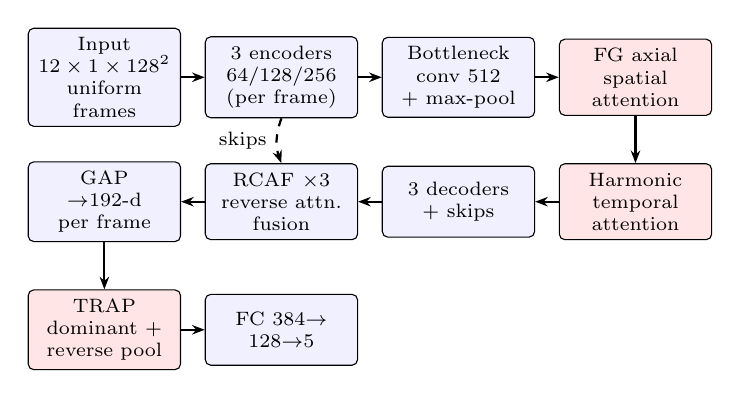
\begin{tikzpicture}[node distance=3mm and 3mm,
  b/.style={draw, rounded corners=2pt, align=center, font=\scriptsize,
            minimum height=9mm, text width=17mm, fill=blue!6},
  a/.style={b, fill=red!10},
  arr/.style={-{Stealth[length=1.6mm]}, thick}]
\node[b] (in) {Input\\$12\times1\times128^2$\\uniform frames};
\node[b, right=of in] (enc) {3 encoders\\64/128/256\\(per frame)};
\node[b, right=of enc] (bot) {Bottleneck\\conv 512\\+ max-pool};
\node[a, right=of bot] (ax) {FG axial\\spatial\\attention};
\node[a, below=6mm of ax] (hp) {Harmonic\\temporal\\attention};
\node[b, left=of hp] (dec) {3 decoders\\+ skips};
\node[b, left=of dec] (rcaf) {RCAF $\times3$\\reverse attn.\\fusion};
\node[b, left=of rcaf] (gap) {GAP\\$\rightarrow$192-d\\per frame};
\node[a, below=6mm of gap] (trap) {TRAP\\dominant +\\reverse pool};
\node[b, right=of trap] (fc) {FC 384$\rightarrow$\\128$\rightarrow$5};
\draw[arr] (in)--(enc); \draw[arr] (enc)--(bot); \draw[arr] (bot)--(ax);
\draw[arr] (ax)--(hp); \draw[arr] (hp)--(dec); \draw[arr] (dec)--(rcaf);
\draw[arr] (rcaf)--(gap); \draw[arr] (gap)--(trap); \draw[arr] (trap)--(fc);
\draw[arr, dashed] (enc.south) to[bend right=20] node[font=\scriptsize, left]{skips} (rcaf.north);
\end{tikzpicture}}
\caption{Initial architecture, ST-CRANet (6.59\,M parameters). Red: modules
added to CRA-Net.}
\label{fig:init_arch}
\end{figure}

\subsection{Final Architecture and Complete System (AnatoPhaseNet v6)}
Fig.~\ref{fig:final_arch} shows the complete final system, from video to the
three outputs, with tensor shapes. Sec.~\ref{sec:changes} explains each block.

\begin{figure*}[!t]
\centering
\resizebox{\textwidth}{!}{%
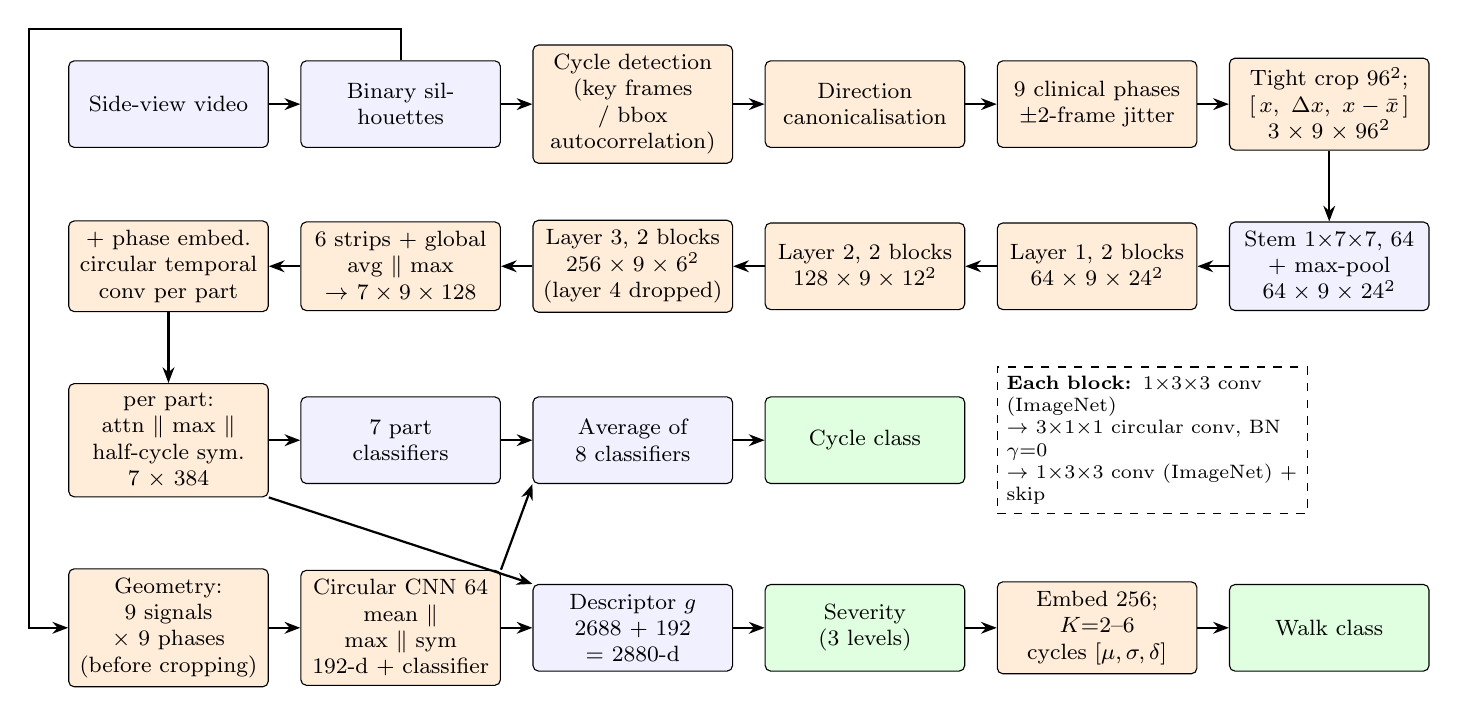
\begin{tikzpicture}[node distance=4mm and 4mm,
  b/.style={draw, rounded corners=2pt, align=center, font=\footnotesize,
            minimum height=11mm, text width=23mm, fill=blue!6},
  n/.style={b, fill=orange!15},
  o/.style={b, fill=green!12},
  arr/.style={-{Stealth[length=2mm]}, thick}]
% ---- row 1: pre-processing
\node[b] (vid) {Side-view video};
\node[b, right=of vid] (sil) {Binary silhouettes};
\node[n, right=of sil] (cyc) {Cycle detection\\(key frames / bbox\\autocorrelation)};
\node[n, right=of cyc] (can) {Direction\\canonicalisation};
\node[n, right=of can] (ph) {9 clinical phases\\$\pm2$-frame jitter};
\node[n, right=of ph] (crop) {Tight crop $96^2$;\\$[\,x,\ \Delta x,\ x-\bar x\,]$\\$3\times9\times96^2$};
% ---- row 2: backbone
\node[b, below=9mm of crop] (stem) {Stem $1{\times}7{\times}7$, 64\\+ max-pool\\$64\times9\times24^2$};
\node[n, left=of stem] (l1) {Layer 1, 2 blocks\\$64\times9\times24^2$};
\node[n, left=of l1] (l2) {Layer 2, 2 blocks\\$128\times9\times12^2$};
\node[n, left=of l2] (l3) {Layer 3, 2 blocks\\$256\times9\times6^2$\\(layer 4 dropped)};
\node[n, left=of l3] (part) {6 strips + global\\avg $\Vert$ max\\$\rightarrow 7\times9\times128$};
\node[n, left=of part] (tc) {+ phase embed.\\circular temporal\\conv per part};
% ---- row 3: part head and outputs
\node[n, below=9mm of tc] (pool) {per part:\\attn $\Vert$ max $\Vert$\\half-cycle sym.\\$7\times384$};
\node[b, right=of pool] (pc) {7 part\\classifiers};
\node[b, right=of pc] (avg) {Average of\\8 classifiers};
\node[o, right=of avg] (out1) {Cycle class};
\node[draw, dashed, align=left, font=\scriptsize, right=of out1, text width=37mm] (blk)
 {\textbf{Each block:} $1{\times}3{\times}3$ conv (ImageNet)\\
  $\rightarrow$ $3{\times}1{\times}1$ circular conv, BN $\gamma{=}0$\\
  $\rightarrow$ $1{\times}3{\times}3$ conv (ImageNet) $+$ skip};
% ---- row 4: geometry branch, descriptor, severity and walk heads
\node[n, below=9mm of pool] (geo) {Geometry: 9 signals\\$\times$ 9 phases\\(before cropping)};
\node[n, right=of geo] (gc) {Circular CNN 64\\mean $\Vert$ max $\Vert$ sym\\192-d + classifier};
\node[b, right=of gc] (desc) {Descriptor $g$\\2688 + 192\\= 2880-d};
\node[o, right=of desc] (sev) {Severity\\(3 levels)};
\node[n, right=of sev] (mc) {Embed 256; $K$=2--6\\cycles $[\mu,\sigma,\delta]$};
\node[o, right=of mc] (walk) {Walk class};
% ---- arrows
\draw[arr] (vid)--(sil); \draw[arr] (sil)--(cyc); \draw[arr] (cyc)--(can);
\draw[arr] (can)--(ph); \draw[arr] (ph)--(crop); \draw[arr] (crop)--(stem);
\draw[arr] (stem)--(l1); \draw[arr] (l1)--(l2); \draw[arr] (l2)--(l3);
\draw[arr] (l3)--(part); \draw[arr] (part)--(tc); \draw[arr] (tc)--(pool);
\draw[arr] (pool)--(pc); \draw[arr] (pc)--(avg); \draw[arr] (avg)--(out1);
\draw[arr] (sil.north) -- ++(0,4mm) -| ([xshift=-5mm]vid.west) |- (geo.west);
\draw[arr] (geo)--(gc); \draw[arr] (gc)--(desc);
\draw[arr] (gc.north east) -- (avg.south west);
\draw[arr] (pool.south east) -- (desc.north west);
\draw[arr] (desc)--(sev); \draw[arr] (sev)--(mc); \draw[arr] (mc)--(walk);
\end{tikzpicture}}
\caption{Final architecture and complete system (AnatoPhaseNet v6, 5.0\,M
parameters). Orange: components introduced in this work. An optional
subject-adversarial classifier (gradient reversal) attaches to $g$ during
training.}
\label{fig:final_arch}
\end{figure*}

\subsection{Target Specifications}
Table~\ref{tab:spec} gives the targets and the values reached by the final model.

\begin{table}[!t]
\centering
\caption{Target specifications (GAIT-IT, 10-fold subject-exclusive)}
\label{tab:spec}
\begin{tabular}{@{}lll@{}}
\toprule
Parameter & Target & Achieved (v6) \\
\midrule
Protocol & subject-exclusive & 10-fold, no leakage \\
Cycle accuracy & $\geq 95\,\%$ & 95.47\,\% \\
Cycle macro-F1 & $\geq 0.95$ & 0.962 \\
Walk accuracy & $\geq 96\,\%$ & 96.28\,\% \\
Worst fold & $\geq 90\,\%$ & 87.4\,\% (open) \\
Severity accuracy & $\geq 80\,\%$ & 80.68\,\% \\
Parameters & $\leq 6$\,M & 4.996\,M \\
Input & 9 frames, $96^2$ & 9 frames, $96^2$ \\
Hardware & 4\,GB GPU & RTX 3050 Laptop, 4\,GB \\
\bottomrule
\end{tabular}
\end{table}

% =====================================================================
\section{Work Carried Out}
\label{sec:changes}
% =====================================================================
\subsection{Data and Protocol}
\textbf{GAIT-IT}~\cite{albuquerque2021} has 21 subjects and 828 side-view
silhouette sequences of five gait types at two impairment levels. From the
provided key-frame annotations we obtain $N=3813$ cycles (normal 202, diplegic
846, hemiplegic 780, neuropathic 729, Parkinsonian 1256).
\textbf{INIT}~\cite{ortells2018} has 10 subjects and 160 sequences of eight
styles; with our cycle detector it yields 589 usable cycles. Sec.~\ref{sec:c4}
describes the detector.

\textbf{Change 0 -- evaluation protocol.} ST-CRANet was trained on a random,
class-stratified 70/15/15 split of \emph{sequences}, so every subject was present
in training, validation and test. All later models use 10 subject-exclusive
folds. Let $\mathcal{S}$ be the set of subjects, partitioned into
$\mathcal{S}_1,\dots,\mathcal{S}_{10}$ with
$\mathcal{S}_i\cap\mathcal{S}_j=\emptyset$. Fold $k$ tests on $\mathcal{S}_k$,
validates on $\mathcal{S}_{k+1}$ and trains on the rest, with split seed 42
fixed for all versions. Each row of Table~\ref{tab:prog} therefore uses the
same test subjects, and accuracy differences are caused by the model alone.

\subsection{Initial Model and Why It Failed}
ST-CRANet reached 100\,\% training accuracy but only 77.24\,\% validation
accuracy (macro-F1 0.788) on the leaky split. Two causes were identified.

\emph{(a) Uniform sampling destroys phase correspondence.} A walk of $L$ frames
with cycle period $P$ contains $L/P$ cycles. Uniform sampling takes frame
$i\cdot\frac{L-1}{T-1}$, whose gait phase is
$\phi_i=\big(i\frac{L-1}{T-1}\bmod P\big)/P$. This depends on $L$ and $P$, so
the $i$-th input frame shows a different phase in every sequence (and at a
different walking speed). The temporal attention therefore has to learn an
alignment that changes from sample to sample.

\emph{(b) Too few, too large samples.} 828 sequences for 6.59\,M parameters,
with a 2D encoder that sees frame appearance, invite memorisation of individuals.

\subsection{Change 1 -- Clinical Phase Alignment (ST-PhaseNet)}
\textbf{What.} Each walk is cut into gait cycles, and each cycle is represented
by its nine key frames, from initial contact through mid-stance, terminal
stance, pre-swing, initial, mid- and terminal swing to cycle completion.

\textbf{Why (speed invariance).} Let $x(t)$ be a walk and $x_\alpha(t)=x(\alpha
t)$ the same walk at speed $\alpha$. Key-phase events scale with time,
$\tau^{(\alpha)}_p=\tau_p/\alpha$, so $x_\alpha(\tau^{(\alpha)}_p)=x(\tau_p)$
for every phase $p$. The 9-frame input is exactly invariant to cadence, and
input $p$ always means the same biomechanical event, which removes cause (a). It
also turns 828 sequences into 3813 cycles, a $4.6\times$ increase in samples.

\textbf{Head.} The phase-indexed reverse attention (P-TRAP) head scores each
phase, $s_t$, and pools a dominant and a complementary view:
\begin{equation}
\mathbf{f}_{\text{dom}}=\sum_t \mathrm{softmax}(s)_t\,\mathbf{h}_t,\qquad
\mathbf{f}_{\text{rev}}=\sum_t \mathrm{softmax}(-s)_t\,\mathbf{h}_t .
\end{equation}

\textbf{Effect.} 89.10\,\% cycle and 92.72\,\% walk accuracy, now under the
\emph{strict} protocol (Table~\ref{tab:prog}). Initialising the spatial filters
from ImageNet ResNet-18 gave 89.51\,\%.

\subsection{Change 2 -- Anatomical Decomposition (v1--v3)}
v1 split the feature map into an upper (trunk, top 40\,\%) and a lower (legs,
60\,\%) region and added a flip asymmetry
$\mathbf{a}=|\mathbf{h}-\mathrm{flip}_W(\mathbf{h})|$: 91.08\,\%. v2 cropped
every frame to its bounding box before resizing to $96^2$. A subject of height
$h_{\text{box}}$ in a frame of height $H$ is magnified by $H/h_{\text{box}}$,
which raised limb resolution from about 35 to 85 pixels: 93.34\,\%. v3 added a
lower-body asymmetry, a trunk-mobility term and focal loss with label smoothing
$\varepsilon=0.05$:
\begin{equation}
\mathcal{L}_{\text{FL}}=-\textstyle\sum_c (1-p_c)^{\gamma}\,
\tilde{y}_c\log p_c,\quad
\tilde{y}_c=\begin{cases}1-\varepsilon & c=y\\ \frac{\varepsilon}{K-1}&
\text{else}\end{cases}
\end{equation}
with $\gamma=1.5$, which down-weights easy cycles. v3 reached 93.01\,\%, but
fold 3 (79.9\,\%) and fold 9 (86.6\,\%) stayed weak and training accuracy hit
99.96\,\%. The remaining gap was generalisation, not capacity.

\subsection{Change 3 -- Diagnosis of v3 and the v4 Redesign}
\label{sec:c4}
Inspecting v3's code and data showed six concrete defects. Each was fixed as
follows.

\textbf{(i) Mirrored walking directions $\rightarrow$ canonicalisation.} The
correlation between mean silhouettes of GAIT-IT \texttt{\_front} and
\texttt{\_back} walks is 0.65 as recorded and \textbf{0.996} after a horizontal
flip, so $x_{\text{back}}\approx M x_{\text{front}}$ with $M$ the mirror
operator. A side-view body is not left--right symmetric, because a walker faces
one way. For every subject, $|\mathbf{h}-\mathrm{flip}_W(\mathbf{h})|$ is
therefore dominated by the facing direction and not by limb asymmetry: v3's
asymmetry feature mostly encoded \emph{direction}. We flip every right-to-left
walk at cache time ($\tilde{x}=Mx$), so all cycles share one direction and the
network does not spend capacity learning two mirrored copies of each class.

\textbf{(ii) Partial transfer $\rightarrow$ full inflation with an exact
identity start.} v3 copied only \texttt{conv1} of the first block of each stage,
loaded no BN statistics, and fed a frame-difference channel through ImageNet
green-channel filters. v4 copies \emph{all} conv and BN tensors of the ResNet-18~\cite{he2016resnet}
stem and layers 1--3. Each 2D kernel $W\in\R^{C'\times C\times k\times k}$
becomes $W'\in\R^{C'\times C\times 1\times k\times k}$ with $W'_{:,:,0}=W$. A
3D convolution with temporal extent 1 applies $W$ to every phase independently,
so the inflated layer equals the 2D layer frame by frame. Each block adds a
temporal residual branch:
\begin{equation}
\mathbf{u}=\mathrm{ReLU}(\mathrm{BN}_1(W_1*\mathbf{x})),\
\mathbf{v}=\mathrm{ReLU}\big(\mathbf{u}+\mathrm{BN}_t(W_t\circledast\mathbf{u})\big).
\end{equation}
\begin{proposition}
If $\mathrm{BN}_t$ is initialised with $\gamma=0,\beta=0$, the (2+1)D network
equals the pretrained 2D ResNet-18 applied to each phase at initialisation.
\end{proposition}
\begin{proof}
$\mathrm{BN}_t(z)=\gamma\hat{z}+\beta=0$, so
$\mathbf{v}=\mathrm{ReLU}(\mathbf{u})=\mathbf{u}$, since
$\mathbf{u}\ge 0$. The block reduces to the two inflated spatial convolutions
plus the shortcut, i.e.\ the 2D BasicBlock per phase. By induction over blocks,
the same holds for the whole network.
\end{proof}
Training therefore starts from the full ImageNet solution and only \emph{adds}
temporal modelling as $\gamma$ grows.

\textbf{(iii) Zero padding of a periodic signal $\rightarrow$ circular
convolution.} After cycle completion the next initial contact follows, so the
phase index lives on $\mathbb{Z}_T$. Zero padding creates artificial edges at
$t=0$ and $t=T-1$. With circular padding
$(W\circledast\mathbf{u})_t=\sum_{j=-1}^{1}W_j\,\mathbf{u}_{(t+j)\bmod T}$. For
a cyclic shift $S_r\mathbf{u}_t=\mathbf{u}_{(t+r)\bmod T}$,
\begin{equation}
(W\circledast S_r\mathbf{u})_t=\textstyle\sum_j W_j\,\mathbf{u}_{(t+j+r)\bmod T}
=(S_r(W\circledast\mathbf{u}))_t ,
\end{equation}
so the operation is shift-equivariant on the cycle. No phase is treated as a
boundary, and the result does not depend on where the cycle is cut.

\textbf{(iv) $3\times3$ map $\rightarrow$ $6\times6$ map and body strips.} With
stride 32 at 96\,px the map was $3\times3$, so the upper/lower split was 1 row
versus 2. Dropping layer 4 gives stride 16 and a $6\times6$ map, enough for six
horizontal body strips plus a global part (GaitSet-style~\cite{chao2019gaitset}).
Each part $p$ gets its own projection to 128-d.

\textbf{(v) Bilateral symmetry in time, not in the image.} In a sagittal view
the two legs overlap in projection. In a symmetric gait the silhouette half a
cycle later shows the other leg in the same configuration, so
$\mathbf{f}_t\approx\mathbf{f}_{t+T/2}$. A unilateral impairment (hemiplegia)
breaks this equality. For $T=9$ phases ($h=\lfloor (T-1)/2\rfloor=4$):
\begin{equation}
\mathbf{s}_p=\tfrac{1}{h}\textstyle\sum_{t=0}^{h-1}\big|\mathbf{f}_{p,t}-\mathbf{f}_{p,t+h}\big| ,
\end{equation}
which is $\approx 0$ for a symmetric walker and grows with asymmetry. Each part
descriptor is $[\text{attention pool}\ \Vert\ \text{max pool}\ \Vert\ \mathbf{s}_p]
\in\R^{384}$.

\textbf{(vi) Over-parameterised head $\rightarrow$ part ensemble.} v3's head
had a 2560-d input containing linear combinations of other features
($\mathbf{h}_u-\mathbf{h}_l$, velocity) and a 5120$\rightarrow$256 FC layer
(about 3\,M parameters for about 17 training subjects). v4 uses one small classifier per
part and averages them, $\bar{\mathbf{z}}=\frac{1}{P}\sum_p\mathbf{z}_p$. If the
part logits have variance $\sigma^2$ and pairwise correlation $\rho$,
\begin{equation}
\mathrm{Var}(\bar{z})=\sigma^2\Big(\rho+\frac{1-\rho}{P}\Big)\le\sigma^2 ,
\end{equation}
so averaging can only reduce variance, with equality only when $\rho=1$. An
auxiliary loss on every part (weight 0.5) keeps each part discriminative.

\textbf{Further changes.} The input has three channels per phase: the
silhouette, the cyclic motion $x_t-x_{(t-1)\bmod T}$, and the deviation from
the cycle's GEI $x_t-\frac1T\sum_\tau x_\tau$. Augmentation adds $\pm2$-frame
phase jitter, $3\times3$ dilation/erosion noise and cycle-consistent erasing.
Class sampling uses probability $\propto n_c^{-1/2}$ per sample, so the expected
share of class $c$ is $n_c\cdot n_c^{-1/2}/Z=\sqrt{n_c}/Z$. The
Parkinsonian:normal ratio falls from $1256/202=6.2$ to $\sqrt{6.2}=2.5$
without the over-correction of hard inverse weights. At test time logits are
averaged over the three jitter views, and a walk is labelled by
$\arg\max_c\frac1{|C|}\sum_{i\in C}\log p_{i,c}$. INIT has no key frames.
There, the cycle period comes from the autocorrelation peak (40--110 frames) of
the bounding-box aspect ratio, and cycles are cut at alternate step peaks.

\textbf{Effect.} Mean accuracy rose from 93.01 to 94.05\,\%, the fold std
fell from 5.38 to 4.04, and fold 3 improved from 79.9 to 90.9\,\%
(Table~\ref{tab:folds}). Fold 9 did not improve (86.6$\rightarrow$85.6\,\%). The
TSM ablation (2D ResNet with cyclic temporal shift, 3.6\,M parameters) gave
94.04\,\% with a lower std (3.30), which confirms that most of the gain comes
from the data and head fixes, not from the backbone type.

\subsection{Change 4 -- Severity and Stride Variability (v5)}
\textbf{Severity multi-task.} A linear head on the descriptor $\mathbf{g}$
predicts normal / mild (\texttt{lvl1}) / severe (\texttt{lvl2}). Severity labels
cost nothing to obtain and force $\mathbf{g}$ to encode \emph{how much} a gait
deviates, not only \emph{how}.

\textbf{Multi-cycle variability.} Stride-to-stride variability is a clinical
marker, especially in Parkinson's disease. During training, $K\in\{2,\dots,6\}$
consecutive cycles of one walk are embedded, $\mathbf{e}_k\in\R^{256}$, and the
walk is classified from
\begin{equation}
\boldsymbol\mu=\tfrac1K\textstyle\sum_k\mathbf{e}_k,\quad
\boldsymbol\sigma=\sqrt{\tfrac1{K-1}\sum_k(\mathbf{e}_k-\boldsymbol\mu)^2},\quad
\boldsymbol\delta=\tfrac1{K-1}\sum_k|\mathbf{e}_{k+1}-\mathbf{e}_k| .
\end{equation}
$\boldsymbol\sigma$ measures overall variability and $\boldsymbol\delta$
measures cycle-to-cycle change; both are zero for a perfectly regular walk.
The total loss is
$\mathcal{L}=\mathcal{L}_{\text{FL}}(\bar{\mathbf z})+0.5\,\mathcal{L}_{\text{part}}
+0.3\,\mathcal{L}_{\text{sev}}+1.0\,\mathcal{L}_{\text{walk}}$.

\textbf{Effect.} Walk accuracy rose from 94.57 (v4) to 95.71\,\%, and cycle
accuracy from 94.05 to 94.81\,\%. Severity accuracy is 79.59\,\% with the head
versus 35.96\,\% (chance level) without it, while cycle accuracy is unchanged
(94.76 vs.\ 94.81\,\%), so severity estimation comes for free.

\subsection{Change 5 -- Biomechanical Geometry Branch (v6)}
\textbf{Why.} Cropping and resizing each frame to a fixed height removes all
information carried by the body's \emph{height over time}.
\begin{proposition}
Let $R_t$ map frame $t$'s bounding box of height $h_t$ to height $H$. Any
feature computed from $R_t(x_t)$ is independent of $h_t$.
\end{proposition}
\begin{proof}
$R_t$ scales by $H/h_t$, so the cropped silhouette always has height $H$,
whatever $h_t$ is. Two frames that differ only in vertical scale give identical
inputs, so the network cannot recover $h_t$.
\end{proof}
Crouch, stoop and vertical bob, which separate diplegic from Parkinsonian gait,
are exactly such height signals. v6 therefore measures nine values on the raw
silhouette before cropping: height, width, lower- and upper-body width, head
bob, centroid height, trunk lean, forward mass offset and fill ratio. Each
length is divided by the walk's median height $\tilde h$, e.g.\
$g_1=h_t/\tilde h-1$. If the camera distance or the subject's size scales all
lengths by $s$, then $s h_t/(s\tilde h)=h_t/\tilde h$: the features are
invariant to scale but keep the within-walk dynamics. A two-layer circular
temporal CNN (64 channels) encodes the $9\times9$ signals into
[mean $\Vert$ max $\Vert$ half-cycle symmetry] (192-d). Its classifier is
averaged with the seven part classifiers, and its features are appended to
$\mathbf g$.

\textbf{Effect.} Cycle accuracy 94.81$\rightarrow$\textbf{95.47\,\%}, macro-F1
0.955$\rightarrow$0.962, std 4.63$\rightarrow$4.11, walk accuracy
95.71$\rightarrow$96.28\,\%, severity 79.59$\rightarrow$80.68\,\%. Diplegic
recall, the target of this change, rose from 84.0 to 87.9\,\%, and
diplegic$\rightarrow$Parkinsonian errors fell from 91 to 71.

\subsection{Change 6 -- Subject-Adversarial Training (tested, not kept)}
A subject classifier is attached to $\mathbf g$ through a gradient-reversal~\cite{ganin2015}
layer: identity in the forward pass, $-\lambda\nabla$ in the backward pass,
with $\lambda=0.1\,(2/(1+e^{-10p})-1)$ ramped over training progress $p$. The
backbone thus solves $\min_\theta\max_\psi\big[-\mathcal{L}_{\text{subj}}\big]$,
i.e.\ it removes identity cues. \textbf{Effect:} 95.16\,\% cycle accuracy (vs.\
95.47) and fold 9 86.3\,\% (vs.\ 87.4), so no gain; it stays switched off.

\subsection{Training Setup}
PyTorch with mixed precision; AdamW, learning rate $10^{-3}$ (backbone
$0.3\times$), weight decay 0.05; 20 epochs, batch 16; EMA of the weights (0.98).
The last-epoch EMA model is evaluated. GPU: RTX 3050 Laptop, 4\,GB.

% =====================================================================
\section{Results and Discussion}
% =====================================================================
\begin{table}[!t]
\centering
\caption{Every version on GAIT-IT (10-fold mean $\pm$ std)}
\label{tab:prog}
\setlength{\tabcolsep}{2.5pt}
\begin{tabular}{@{}lcccc@{}}
\toprule
Model & Params & Cycle acc.\,(\%) & F1 & Walk acc.\,(\%) \\
\midrule
ST-CRANet$^\dagger$ & 6.59\,M & 77.24 (val) & 0.788 & -- \\
ST-PhaseNet & -- & $89.10\pm4.56$ & 0.901 & $92.72\pm4.49$ \\
\quad + ImageNet init & -- & $89.51\pm6.60$ & 0.908 & $92.64\pm7.25$ \\
v1 regions & -- & $91.08\pm6.35$ & -- & $93.26\pm6.25$ \\
v2 + crop & -- & $93.34\pm5.31$ & -- & $94.72\pm6.99$ \\
v3 + focal & -- & $93.01\pm5.38$ & 0.937 & $94.54\pm6.63$ \\
v4 TSM & 3.62\,M & $94.04\pm3.30$ & -- & $94.13\pm5.35$ \\
v4 (2+1)D & 4.13\,M & $94.05\pm4.04$ & 0.949 & $94.57\pm5.78$ \\
v5 w/o severity & 4.93\,M & $94.76\pm4.11$ & -- & $95.54\pm6.94$ \\
v5 & 4.93\,M & $94.81\pm4.63$ & 0.955 & $95.71\pm6.37$ \\
v6 + adversary & 5.37\,M & $95.16\pm4.74$ & 0.957 & $96.27\pm5.68$ \\
\textbf{v6} & \textbf{5.00\,M} & $\mathbf{95.47\pm4.11}$ & \textbf{0.962} & $\mathbf{96.28\pm5.72}$ \\
\bottomrule
\multicolumn{5}{@{}l}{\scriptsize $^\dagger$random sequence split (subjects
shared); all other rows subject-exclusive.}
\end{tabular}
\end{table}

\begin{table}[!t]
\centering
\caption{Test accuracy (\%) per fold, GAIT-IT}
\label{tab:folds}
\scriptsize
\setlength{\tabcolsep}{2pt}
\begin{tabular}{@{}lcccccccccc@{}}
\toprule
Fold & 1 & 2 & 3 & 4 & 5 & 6 & 7 & 8 & 9 & 10 \\
\midrule
v3 & 95.5 & 96.0 & 79.9 & 92.3 & 95.1 & 97.9 & 92.8 & 96.2 & 86.6 & 97.8 \\
v4 & 94.0 & 96.8 & 90.9 & 98.9 & 95.4 & 94.8 & 97.8 & 97.2 & 85.6 & 89.2 \\
v5 & 95.3 & 93.7 & 86.3 & 99.2 & 97.9 & 97.9 & 98.1 & 98.2 & 85.9 & 95.5 \\
v6 & 97.4 & 96.0 & 87.6 & 99.2 & 96.1 & 98.4 & 97.2 & 98.2 & 87.4 & 97.1 \\
\bottomrule
\end{tabular}
\end{table}

\begin{table}[!t]
\centering
\caption{Per-class recall (\%) over all test folds, GAIT-IT}
\label{tab:recall}
\setlength{\tabcolsep}{3pt}
\begin{tabular}{@{}lccccc@{}}
\toprule
Model & Normal & Diplegic & Hemipl. & Neurop. & Parkins. \\
\midrule
v4 & 100.0 & 83.8 & 96.7 & 99.5 & 95.9 \\
v5 & 100.0 & 84.0 & 96.9 & 99.6 & 96.7 \\
v6 & 100.0 & \textbf{87.9} & 96.8 & 99.7 & 96.5 \\
\bottomrule
\end{tabular}
\end{table}

\begin{figure}[!t]
\centering
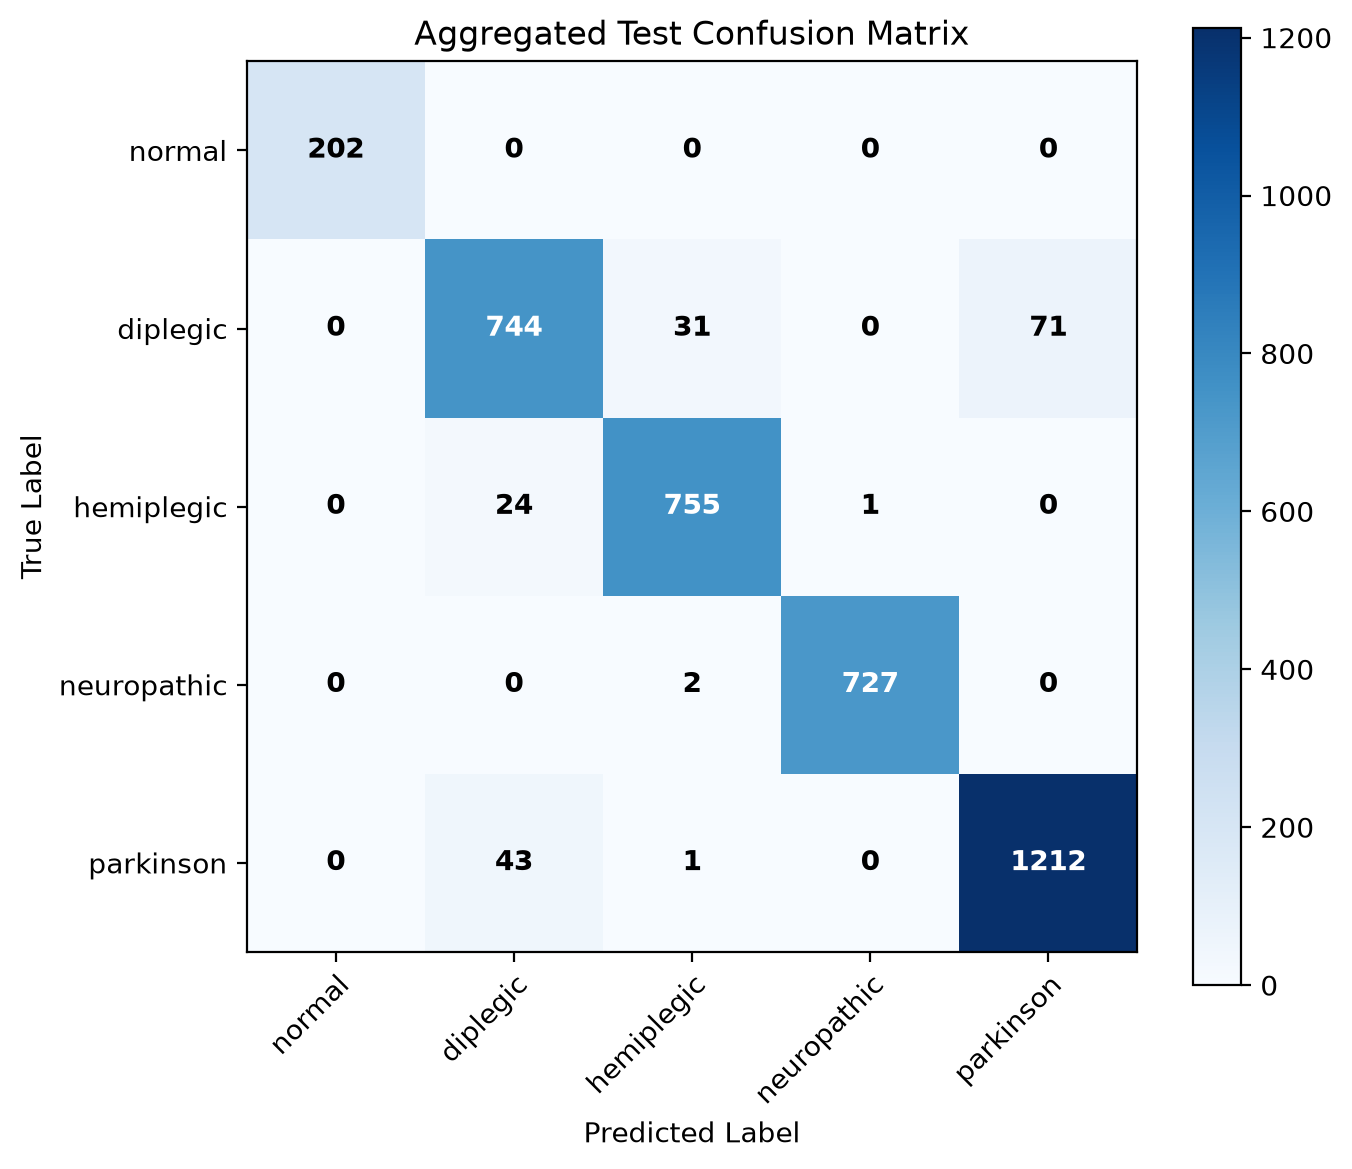
\includegraphics[width=0.82\columnwidth]{cm_gaitit_v6.png}
\caption{Aggregated test confusion matrix of v6 (GAIT-IT, 3813 cycles).}
\label{fig:cm}
\end{figure}

\textbf{Overall progress.} Table~\ref{tab:prog} lists every version. The two
largest steps are phase alignment (Change 1), which went from a model that
failed even with subject leakage to 89.1\,\% without leakage, and anatomical
cropping (v2, +2.3 points). The v4 redesign mainly reduced instability across
subjects (std $-1.3$, fold 3 $+11.0$ points). v5 improved walk-level accuracy,
and the geometry branch of v6 gave the best result on every summary metric.

\textbf{Per class.} Normal, neuropathic, hemiplegic and Parkinsonian cycles are
recognised at $\ge 96.5\,\%$ (Table~\ref{tab:recall}, Fig.~\ref{fig:cm}).
Hemiplegic recall is high from v4 on, as expected from the half-cycle symmetry
term. The remaining error is diplegic$\leftrightarrow$Parkinsonian (71 and 43
cycles). Both gaits are bilateral and symmetric with a flexed posture, so the
symmetry cue cannot separate them, while the posture geometry partly can.

\textbf{Subject dependence.} Folds 3 and 9 are the weakest for every version
(Table~\ref{tab:folds}). The errors are tied to the individual walking styles of
those test subjects, which adversarial identity removal did not fix.

\textbf{Training behaviour.} Fig.~\ref{fig:curves} shows that validation
accuracy saturates within about five epochs. Training accuracy stays below
validation accuracy because training uses jitter, erasing and morphological
noise, while evaluation uses clean inputs with TTA.

\begin{figure}[!t]
\centering
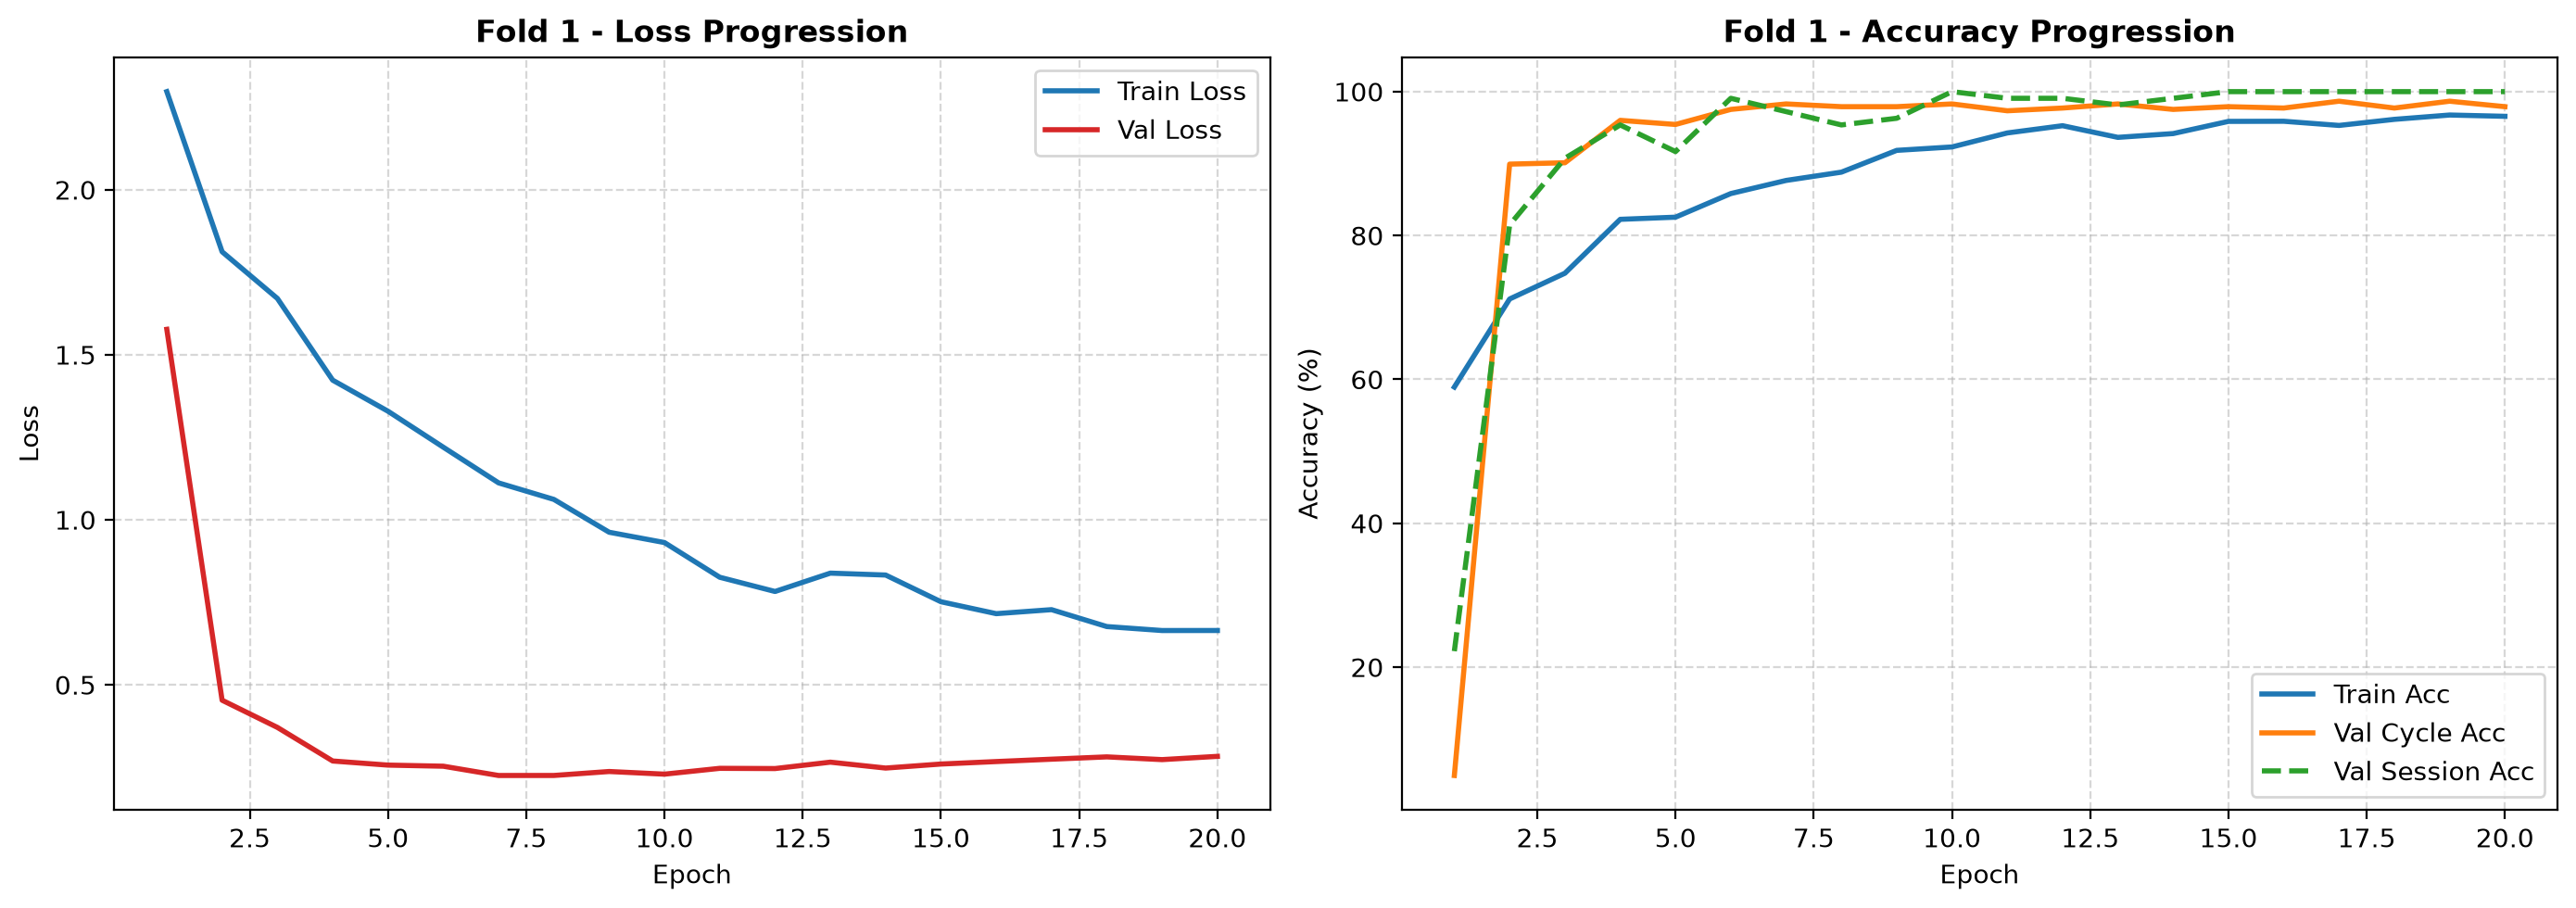
\includegraphics[width=\columnwidth]{curves_v6_fold1.png}
\caption{Loss and accuracy curves of v6, fold 1.}
\label{fig:curves}
\end{figure}

\textbf{INIT.} With leave-one-subject-out folds and detected cycles, v5 reaches
$93.27\pm4.71\,\%$ cycle accuracy (macro-F1 0.919) and 76.56\,\% severity
accuracy on the 6-class protocol (Fig.~\ref{fig:init}). v4 reaches
$93.59\pm4.32\,\%$ on 6 classes and $85.56\pm8.19\,\%$ on 8 classes, where most
errors fall between the two arm-swing levels. A bug in the first cycle detector
had limited v4 on INIT-6 to 88.15\,\%; fixing it gave the +5.4 points.

\begin{figure}[!t]
\centering
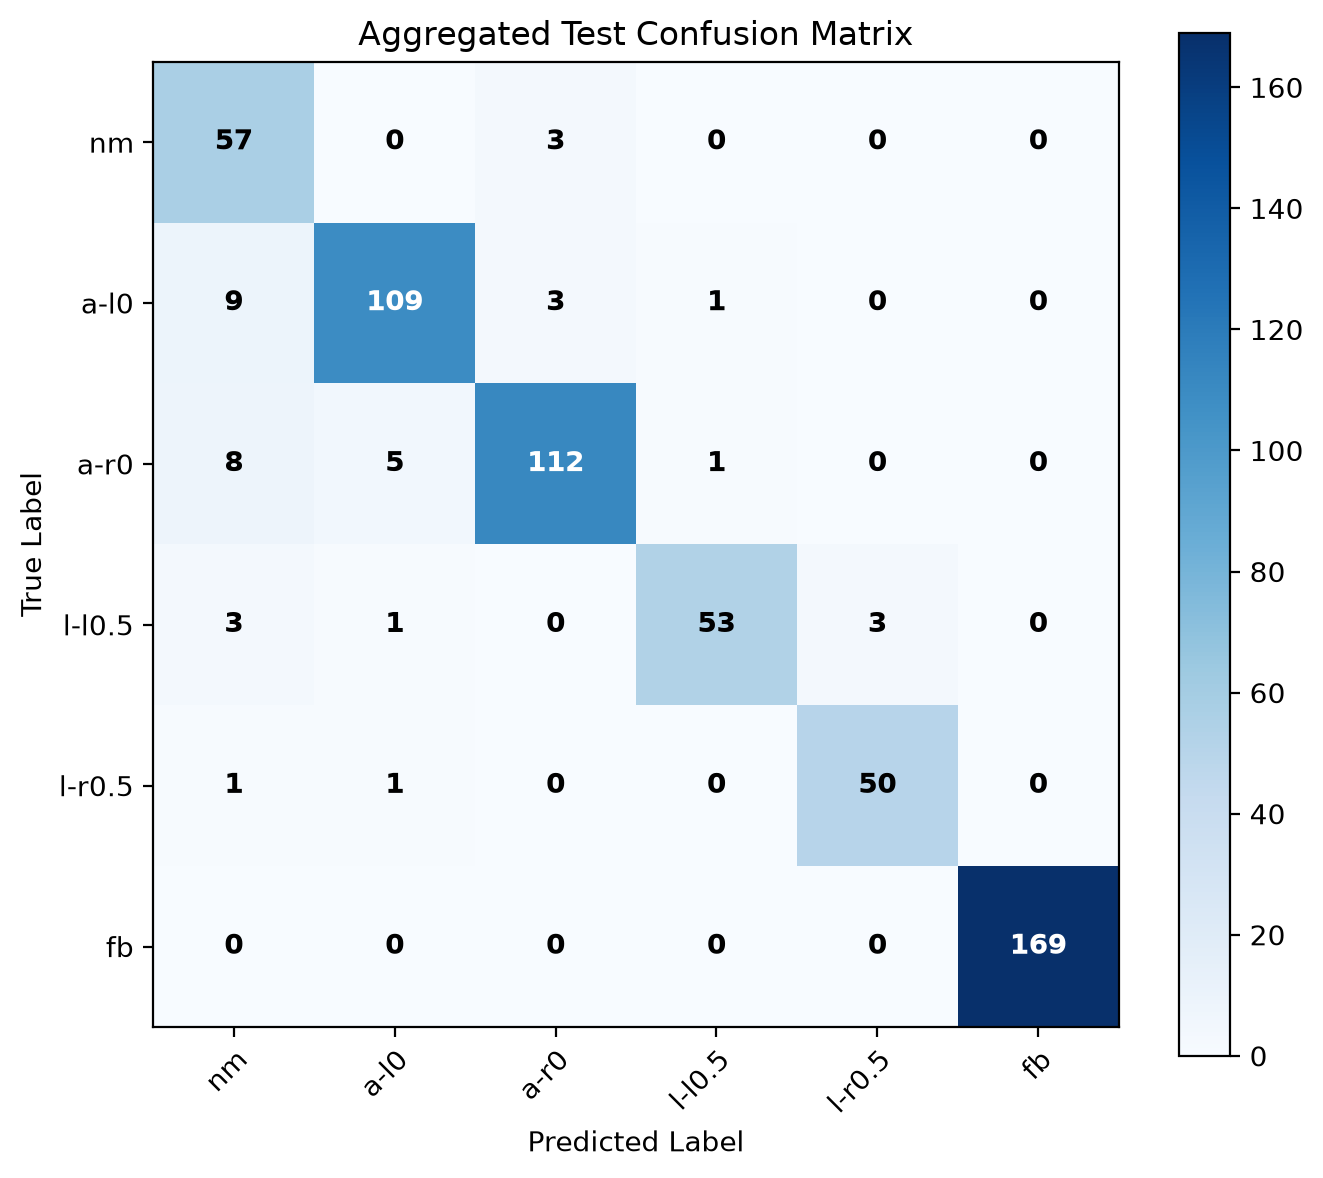
\includegraphics[width=0.78\columnwidth]{cm_init6_v5.png}
\caption{Aggregated test confusion matrix on INIT, 6 classes (v5).}
\label{fig:init}
\end{figure}

\textbf{Comparison with the literature.} CRA-Net's 99.16\,\% on GAIT-IT
\cite{bodepu_cranet} is measured with subjects shared between training and test.
Our extension of it, ST-CRANet, reached only 77.24\,\% even under such a split.
Our 95.47\,\% is measured on unseen subjects, which is the setting that matters
for a new patient, so the numbers are not directly comparable.

\textbf{Limitations.} Both datasets contain \emph{simulated} pathologies
performed by healthy actors. All results use one training seed.

% =====================================================================
\section{Timeline}
% =====================================================================
Table~\ref{tab:time} lists the stages completed so far and the planned work.

\begin{table}[!t]
\centering
\caption{Work completed and planned}
\label{tab:time}
\setlength{\tabcolsep}{3pt}
\begin{tabular}{@{}p{1.6cm}p{4.1cm}p{1.9cm}@{}}
\toprule
Stage & Work & Result \\
\midrule
1 & Literature survey, datasets, ST-CRANet & 77.24\,\% (leaky) \\
2 & Strict protocol; ST-PhaseNet & 89.10\,\% \\
3 & AnatoPhaseNet v1--v3 & 93.34\,\% best \\
4 & v4 redesign, INIT support & 94.05\,\% \\
5 & v5 severity, variability & 94.81\,\% \\
6 & v6 geometry, adversary & 95.47\,\% \\
\midrule
\emph{Next} & \emph{v6 on INIT 6/8; multi-seed runs; ablations of each change} & -- \\
\emph{Next} & \emph{Weak folds 3/9; diplegic vs.\ Parkinsonian; saliency maps} & -- \\
\emph{Final} & \emph{Cross-dataset test; final report and paper} & -- \\
\bottomrule
\end{tabular}
\end{table}

% =====================================================================
\section{Conclusion}
% =====================================================================
Starting from a frame-based CRA-Net extension, we built AnatoPhaseNet through
a sequence of changes, each motivated by an observed failure, justified
analytically and measured on fixed subject-exclusive folds. The final model
reaches 95.47\,\% cycle and 96.28\,\% walk accuracy on GAIT-IT with fewer
parameters than the initial model (5.0 vs.\ 6.6\,M), and 93.3\,\% on INIT-6.
The remaining work targets diplegic--Parkinsonian confusion and the two
subject-specific weak folds.

% =====================================================================
\begin{thebibliography}{99}
\bibitem{dietz2013} V. Dietz, ``Gait disorders,'' \emph{Handb. Clin. Neurol.},
vol.~110, pp.~133--143, 2013.
\bibitem{baker2018} J.~M. Baker, ``Gait disorders,'' \emph{Am. J. Med.},
vol.~131, no.~6, pp.~602--607, 2018.
\bibitem{albuquerque2021} P. Albuquerque, J.~P. Machado, T.~T. Verlekar,
P.~L. Correia, and L.~D. Soares, ``Remote gait type classification system using
markerless 2D video,'' \emph{Diagnostics}, vol.~11, no.~10, p.~1824, 2021.
\bibitem{ortells2018} J. Ortells, M.~T. Herrero-Ezquerro, and R.~A. Mollineda,
``Vision-based gait impairment analysis for aided diagnosis,'' \emph{Med. Biol.
Eng. Comput.}, vol.~56, pp.~1553--1564, 2018.
\bibitem{bodepu_cranet} D. Bodepu, M.~I. Junaid, S. Madarapu, J.~P. Sahoo, and
S. Ari, ``CRA-Net: Cross reverse attention network for classification of
neuro-degenerative diseases based on gait analysis,'' \emph{Biomed. Signal
Process. Control}.
\bibitem{verlekar2018} T.~T. Verlekar, P.~L. Correia, and L.~D. Soares,
``Using transfer learning for classification of gait pathologies,'' in
\emph{Proc. IEEE BIBM}, 2018, pp.~2376--2381.
\bibitem{loureiro2020} J. Loureiro and P.~L. Correia, ``Using a skeleton gait
energy image for pathological gait classification,'' in \emph{Proc. IEEE FG},
2020, pp.~503--507.
\bibitem{hu2018se} J. Hu, L. Shen, and G. Sun, ``Squeeze-and-excitation
networks,'' in \emph{Proc. IEEE CVPR}, 2018, pp.~7132--7141.
\bibitem{woo2018cbam} S. Woo, J. Park, J.-Y. Lee, and I.~S. Kweon, ``CBAM:
Convolutional block attention module,'' in \emph{Proc. ECCV}, 2018, pp.~3--19.
\bibitem{wang2018nonlocal} X. Wang, R. Girshick, A. Gupta, and K. He,
``Non-local neural networks,'' in \emph{Proc. IEEE CVPR}, 2018, pp.~7794--7803.
\bibitem{tran2018r21d} D. Tran, H. Wang, L. Torresani, J. Ray, Y. LeCun, and
M. Paluri, ``A closer look at spatiotemporal convolutions for action
recognition,'' in \emph{Proc. IEEE CVPR}, 2018, pp.~6450--6459.
\bibitem{lin2019tsm} J. Lin, C. Gan, and S. Han, ``TSM: Temporal shift module
for efficient video understanding,'' in \emph{Proc. IEEE ICCV}, 2019,
pp.~7083--7093.
\bibitem{guo2021ssan} X. Guo, X. Guo, and Y. Lu, ``SSAN: Separable
self-attention network for video representation learning,'' in \emph{Proc. IEEE
CVPR}, 2021, pp.~12618--12627.
\bibitem{chao2019gaitset} H. Chao, Y. He, J. Zhang, and J. Feng, ``GaitSet:
Regarding gait as a set for cross-view gait recognition,'' in \emph{Proc.
AAAI}, 2019, pp.~8126--8133.
\bibitem{he2016resnet} K. He, X. Zhang, S. Ren, and J. Sun, ``Deep residual
learning for image recognition,'' in \emph{Proc. IEEE CVPR}, 2016, pp.~770--778.
\bibitem{ganin2015} Y. Ganin and V. Lempitsky, ``Unsupervised domain adaptation
by backpropagation,'' in \emph{Proc. ICML}, 2015, pp.~1180--1189.
\end{thebibliography}

\vspace{6mm}
\noindent\begin{tabular}{@{}l@{}}
\rule{4.5cm}{0.4pt}\\
Signature of Supervisor\\
[[Supervisor Name]]\\
Date: \rule{2.5cm}{0.4pt}
\end{tabular}

\end{document}
